\section{Motivation}

\begin{frame}
	{Motivation}	
	{Image analysis}
	
	The problems we are interested in come from \emph{Image Analysis}.
	
	\pause
	\vspace{1em}

\only<2>{
\begin{minipage}[t][0.25\textheight][t]{\textwidth}
\textbf{Segmentation:} Given input image $f_I:\Omega \rightarrow [0,1]$, find natural number $n$ and partition $\mathcal{I}^{\star} = \{ \Omega_i \subset \Omega \; | \; i \leq n \}$ such that $f_{\widehat{\vec{I}}}$
%
%
\begin{align*}
	\mathcal{I}^{\star} = \argmin_{\mathcal{I}} E_{seg}(\mathcal{I},f_{\vec{I}}) &\quad  \text{subject to } \begin{array}{l}
	\forall i\neq j:\; \Omega_i \cap \Omega_j = \emptyset\\ 
	\bigcup_i^{n} \Omega_i = \Omega
	\end{array}
\end{align*}
%
%
\begin{minipage}{.3\textwidth}
\center
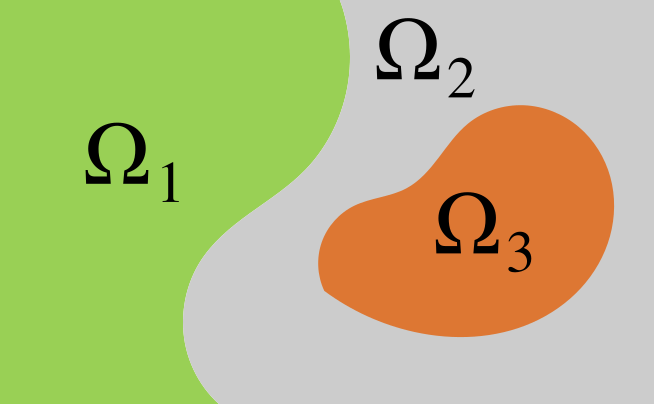
\includegraphics[scale=0.26]{figures/motivation/segmentation-stylised.png}
\end{minipage}
\begin{minipage}{.3\textwidth}
\center
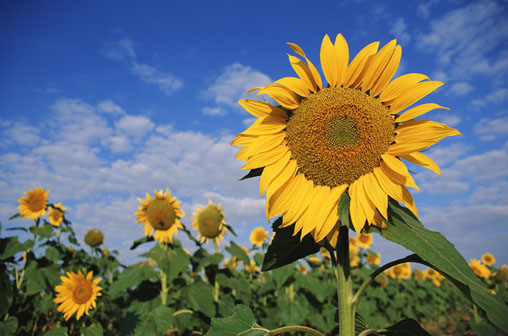
\includegraphics[scale=0.15]{figures/motivation/pock-sunflower.png}
\end{minipage}
\begin{minipage}{.3\textwidth}
\center
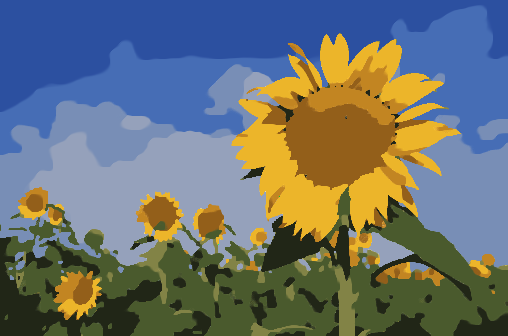
\includegraphics[scale=0.15]{figures/motivation/pock-segmentation.png}
\end{minipage}
\end{minipage}
}
%
%
\onslide<3->{
\begin{minipage}[t][0.13\textheight][t]{\textwidth}
\begin{tabular}{p{0.6\textwidth}p{0.2\textwidth}}
\textbf{Segmentation:} $\mathcal{I}^{\star} = \argmin_{\mathcal{I}} E_{seg}(\mathcal{I},f_{\vec{I}})$ & \raisebox{-.5\height}{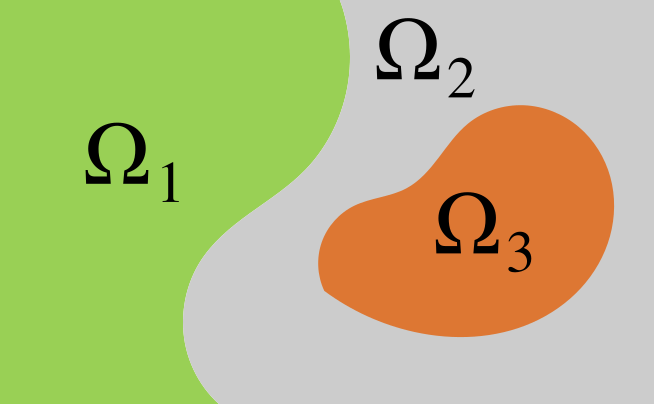
\includegraphics[scale=0.12]{figures/motivation/segmentation-stylised.png}}
\end{tabular}
\end{minipage}
}
%
%
\pause
\only<3>{
\begin{minipage}[t][0.25\textheight][t]{\textwidth}
\textbf{Denoising:} Given a noisy image $f_{\vec{\widetilde{I}}}$ corrupted, find an estimation $f_{\widehat{\vec{I}}}$ of the original image such that
%
%
\begin{align*}
	f_{\widehat{\vec{I}}} &= \argmin_f E_{den}(f,f_{\vec{\widetilde{I}}})
\end{align*}
%
%
\begin{minipage}{.3\textwidth}
\center
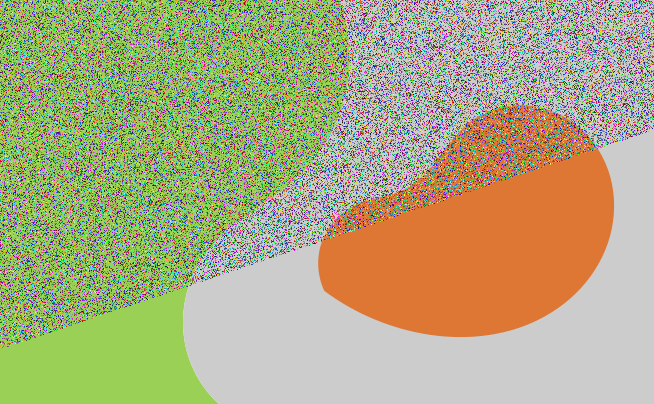
\includegraphics[scale=0.26]{figures/motivation/denoising-stylised.png}
\end{minipage}
\begin{minipage}{.3\textwidth}
\center
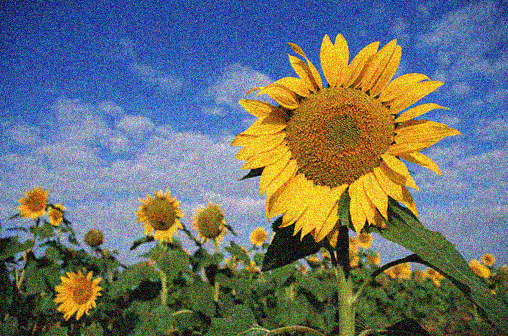
\includegraphics[scale=0.15]{figures/motivation/pock-sunflower-noisy.png}
\end{minipage}
\begin{minipage}{.3\textwidth}
\center
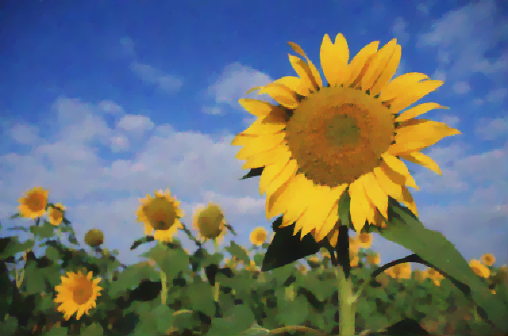
\includegraphics[scale=0.15]{figures/motivation/pock-sunflower-fista-denoising-100.png}
\end{minipage}
\end{minipage}
}
%
\onslide<4->{
\begin{minipage}[t][0.13\textheight][t]{\textwidth}
\begin{tabular}{p{0.6\textwidth}p{0.2\textwidth}}
\textbf{Denoising:} $f_{\widehat{\vec{I}}} = \argmin_f E_{den}(f,f_{\vec{\widetilde{I}}})$ & \raisebox{-.5\height}{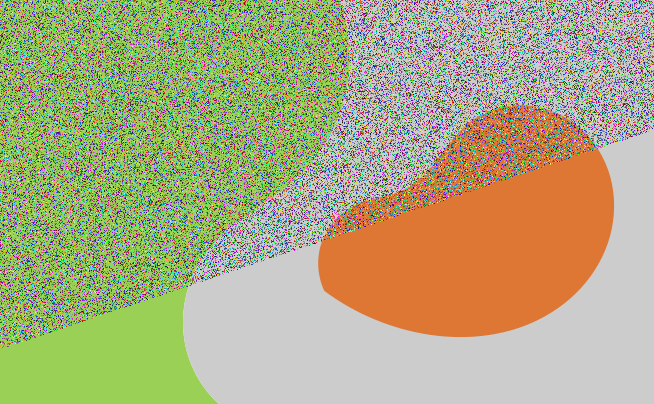
\includegraphics[scale=0.12]{figures/motivation/denoising-stylised.png}}
\end{tabular}
\end{minipage}
}
%
\pause
%
\only<4>{
\begin{minipage}[t][0.25\textheight][t]{\textwidth}
\textbf{Inpainting:} Given an image $f_{\widetilde{\vec{I}}}$ and a collection of missing patches $\mathcal{P}$, complete the patches such that
%
%
\begin{align*}
	f_{\vec{\widehat{I}}} &= \argmin_f E_{inp}(f,f_{\widetilde{\vec{I}}}) \quad \text{subject to}\; f(\Omega \setminus \mathcal{P}) = f_{\widetilde{\vec{I}}}(\Omega \setminus \mathcal{P}).
\end{align*}
%
%
\begin{minipage}{.3\textwidth}
\center

\includegraphics[scale=0.26]{figures/motivation/inpainting-stylised.png}
\end{minipage}
\begin{minipage}{.3\textwidth}
\center
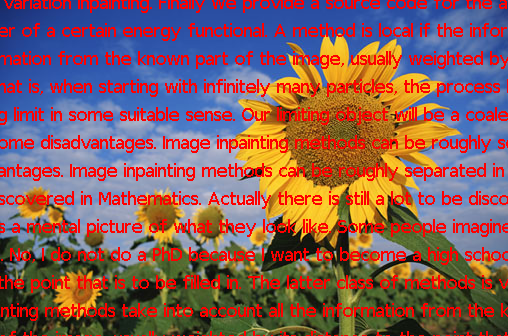
\includegraphics[scale=0.15]{figures/motivation/pock-sunflower-mask.png}
\end{minipage}
\begin{minipage}{.3\textwidth}
\center
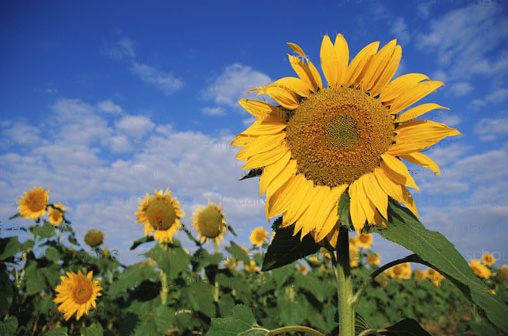
\includegraphics[scale=0.15]{figures/motivation/pock-sunflower-inpainted.png}
\end{minipage}
\end{minipage}
}
%
\pause
%
\onslide<5->{
\begin{minipage}[t][0.13\textheight][t]{\textwidth}
\begin{tabular}{p{0.6\textwidth}p{0.2\textwidth}}
\textbf{Inpainting:} $f_{\vec{\widehat{I}}} = \argmin_f E_{inp}(f,f_{\widetilde{\vec{I}}})$ & \raisebox{-.5\height}{
\includegraphics[scale=0.12]{figures/motivation/inpainting-stylised.png}}
\end{tabular}
\end{minipage}
}
%
%
\only<5>{
\begin{minipage}[t][0.27\textheight][t]{\textwidth}
Energies are defined according to assumptions made about the solution, e.g.,
\begin{itemize}
	\item{ \emph{Data fidelity}. The solution should not differ much from the input. }
	\item{ \emph{Spatial coherence}. Images are composed of regions with low variability in color. }
\end{itemize}
\end{minipage}
}
\end{frame}

\begin{frame}
{Motivation}
{Geometric priors}
The \emph{Mumford Shah} is a model for segmentation and denoising.
%
%
\begin{align*}
	\min_{f,\mathcal{K}} \alpha \int_{\Omega} \norm{ f_{\vec{I}} - f}^2dx + \beta \int_{\Omega \setminus \mathcal{K}} \norm{ \nabla f}^2 dx + \lambda Per(\mathcal{K}).
\end{align*}
%
%
\pause
The \emph{ROF} model uses \emph{Total variation} for image denoising
%
%
\begin{align*}
	\min_{f,\mathcal{K}} \alpha \int_{\Omega} \norm{ f_{\vec{I}} - f}^2dx + \beta \int_{\Omega} \norm{ \nabla f }dx
\end{align*}
%
%
\begin{itemize}
	\item{A measure of length is present in both models.}
	\item{\emph{Geometric priors} as length, area or curvature are useful due to its flexibility and its well stablished results.}
\end{itemize}
%
%
\pause
\vspace{1em}
In this thesis, we are interested in the combined use of \emph{length} and \emph{squared curvature} as geometric priors.
\end{frame}

\begin{frame}
{Motivation}
{Completion property}
\begin{minipage}[t][0.5\textheight][t]{\textwidth}
\only<1->{
\center
$\min_{ \Omega \in \{\Omega_{c}, \Omega_{d} \} } \int_{\partial \Omega}{ds}.$
}
\only<1>{
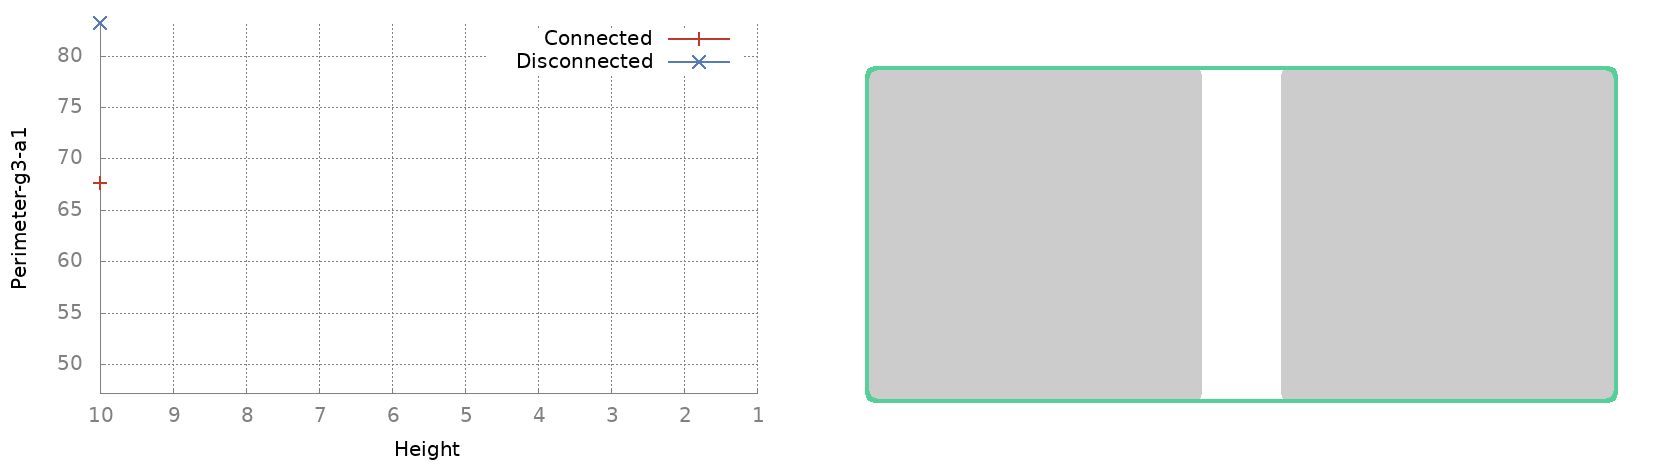
\includegraphics[scale=0.25]{figures/motivation/completion/perimeter-0.png}
}
\only<2>{
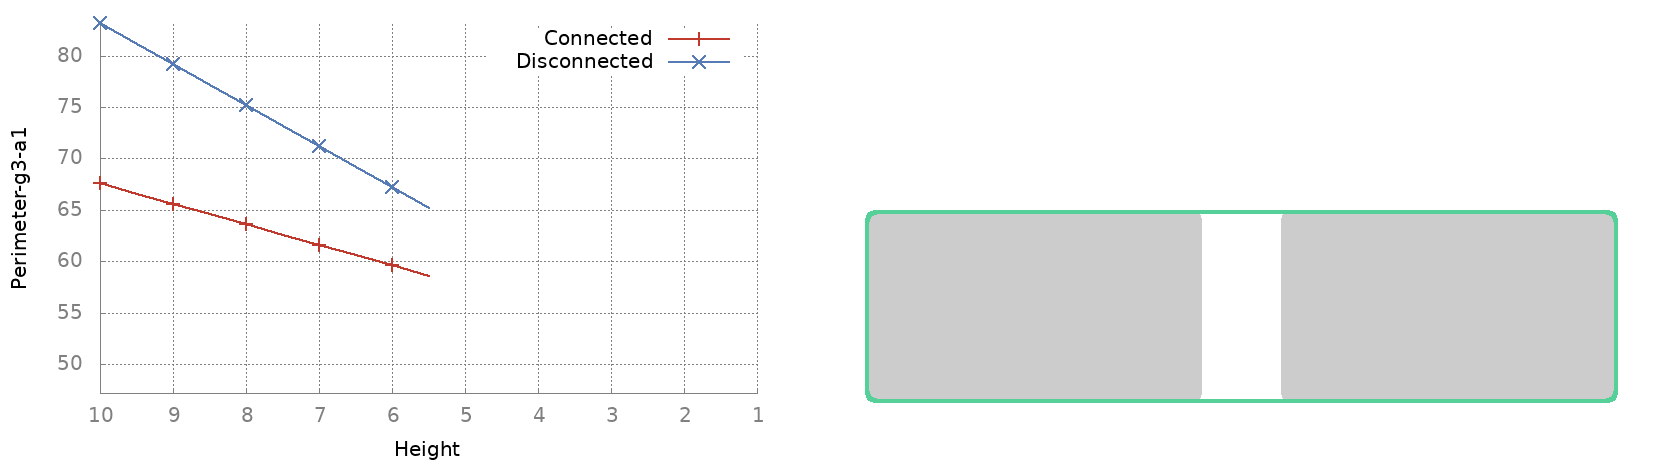
\includegraphics[scale=0.25]{figures/motivation/completion/perimeter-1.png}
}
\only<3>{
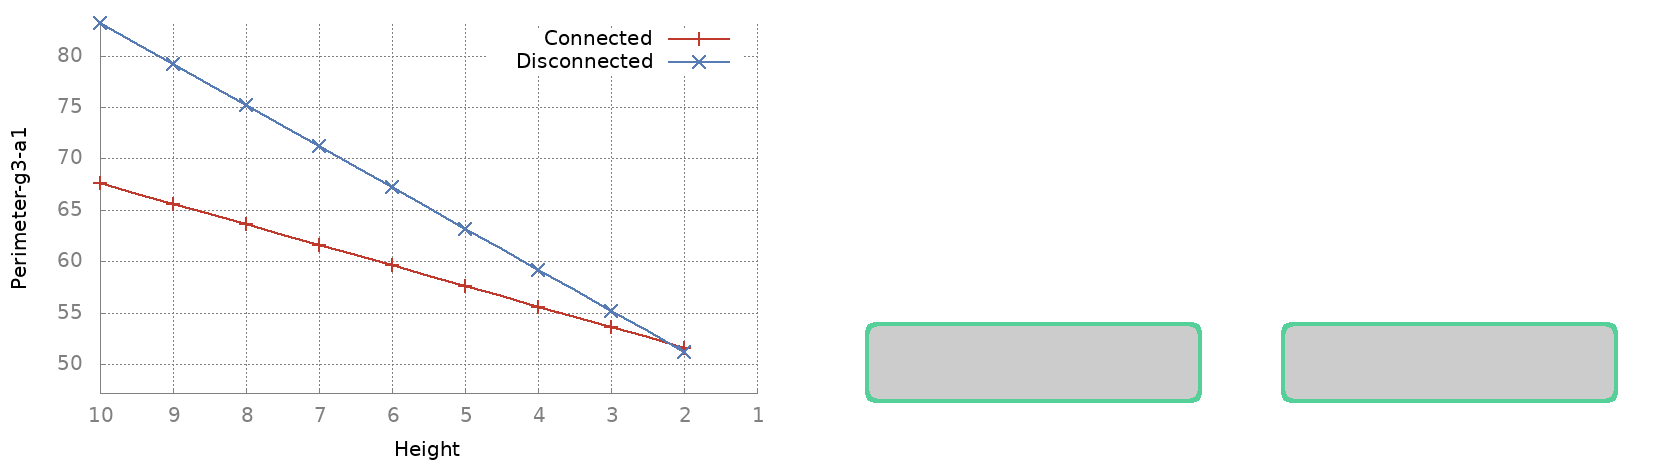
\includegraphics[scale=0.25]{figures/motivation/completion/perimeter-2.png}
}
\only<4->{
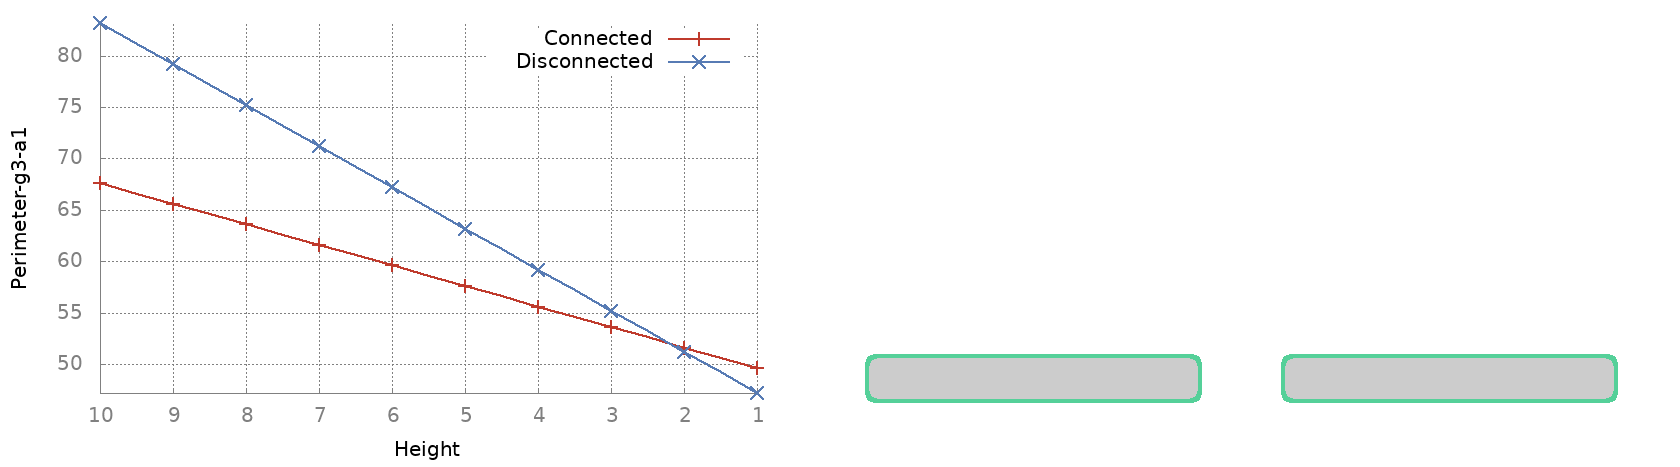
\includegraphics[scale=0.25]{figures/motivation/completion/perimeter-3.png}
}
\end{minipage}
\begin{minipage}[t][0.5\textheight][t]{\textwidth}
\only<5->{
\center
$\min_{ \Omega \in \{\Omega_{c}, \Omega_{d} \} } \int_{\partial \Omega}{ds} + \int_{\partial \Omega}{ \kappa ^2ds}.$}
\only<5>{
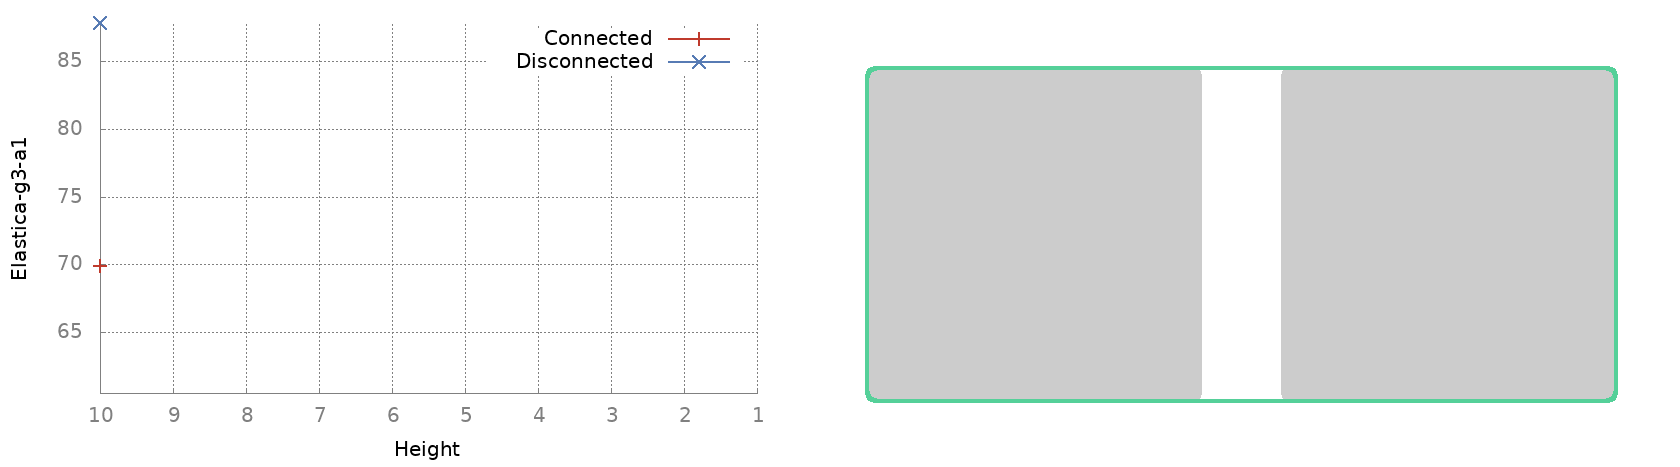
\includegraphics[scale=0.25]{figures/motivation/completion/elastica-0.png}
}
\only<6>{
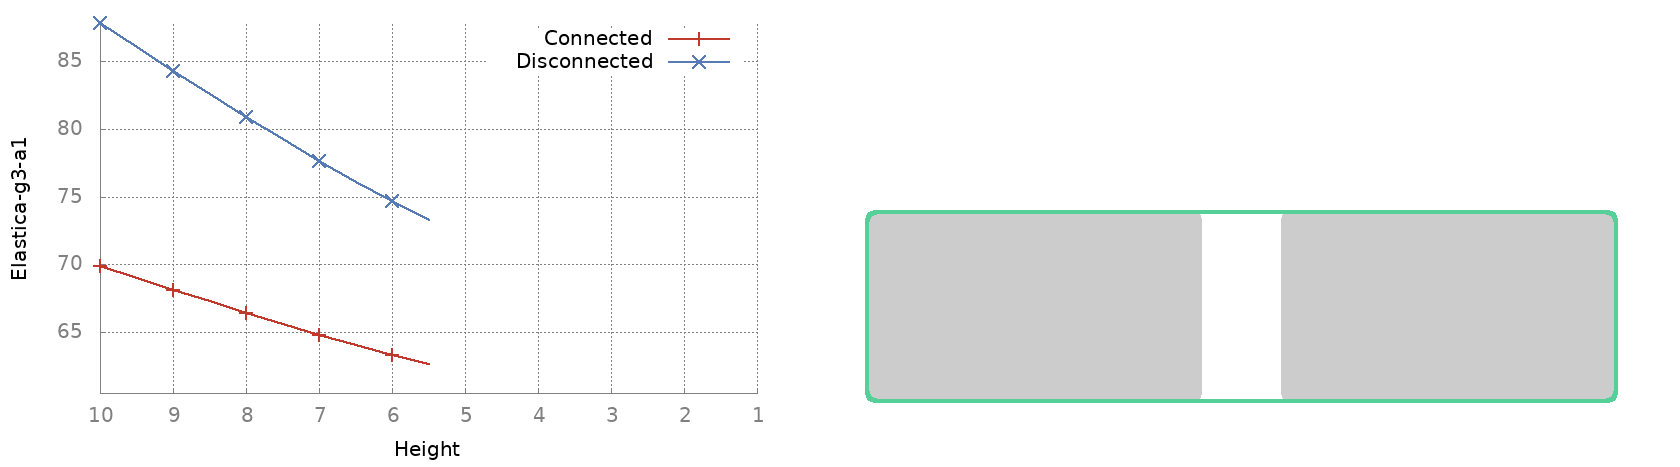
\includegraphics[scale=0.25]{figures/motivation/completion/elastica-1.png}
}
\only<7>{
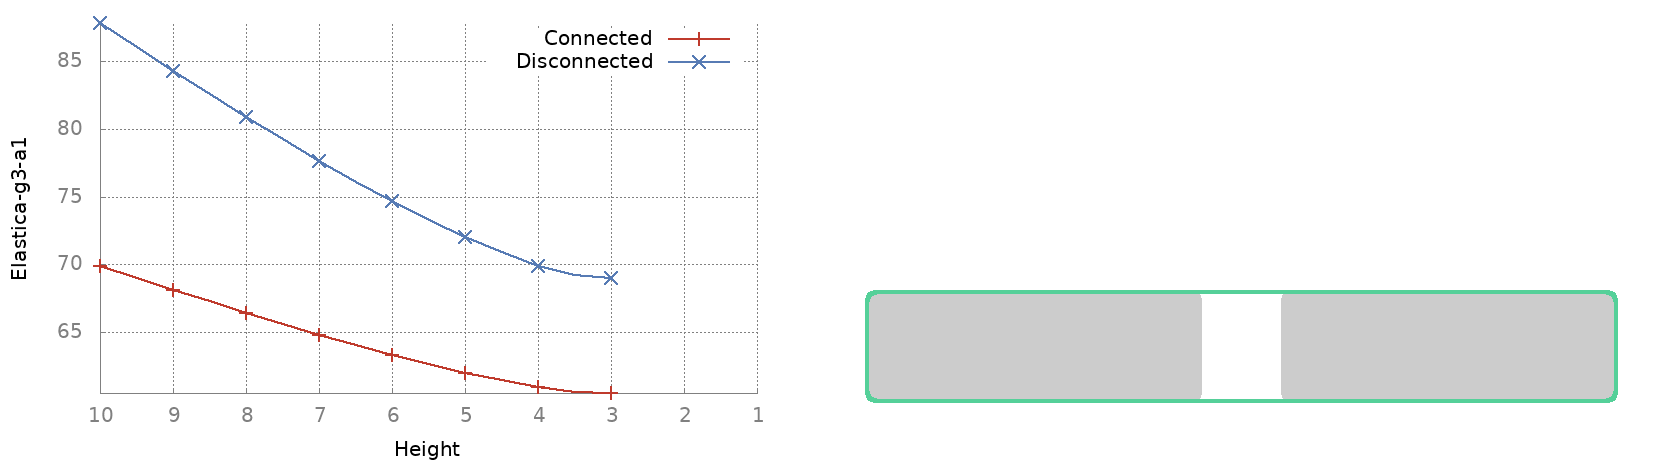
\includegraphics[scale=0.25]{figures/motivation/completion/elastica-2.png}
}
\only<8->{
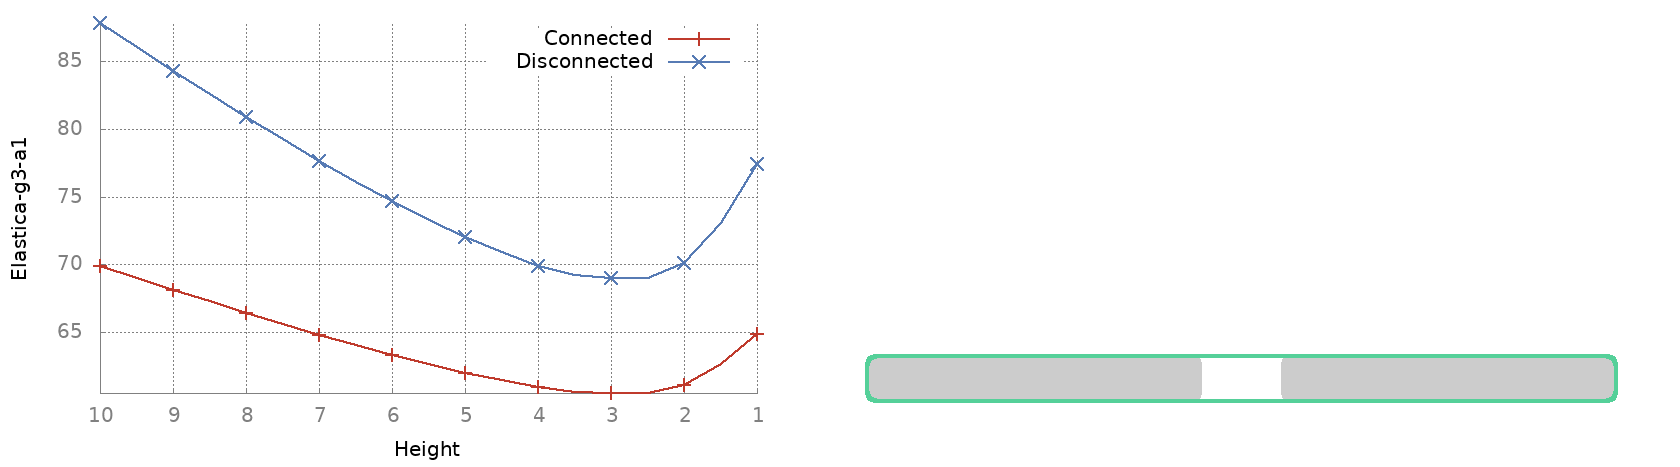
\includegraphics[scale=0.25]{figures/motivation/completion/elastica-3.png}
}
\end{minipage}
\end{frame}

\begin{frame}
{Motivation}
{Completion property}
\begin{minipage}[t][0.5\textheight][t]{\textwidth}
\only<1->{
\center
$\min_{ \Omega \in \{\Omega_{c}, \Omega_{d} \} } \int_{\partial \Omega}{ds} + \int_{\partial \Omega}{ \kappa ^2ds}.$}
\only<1>{
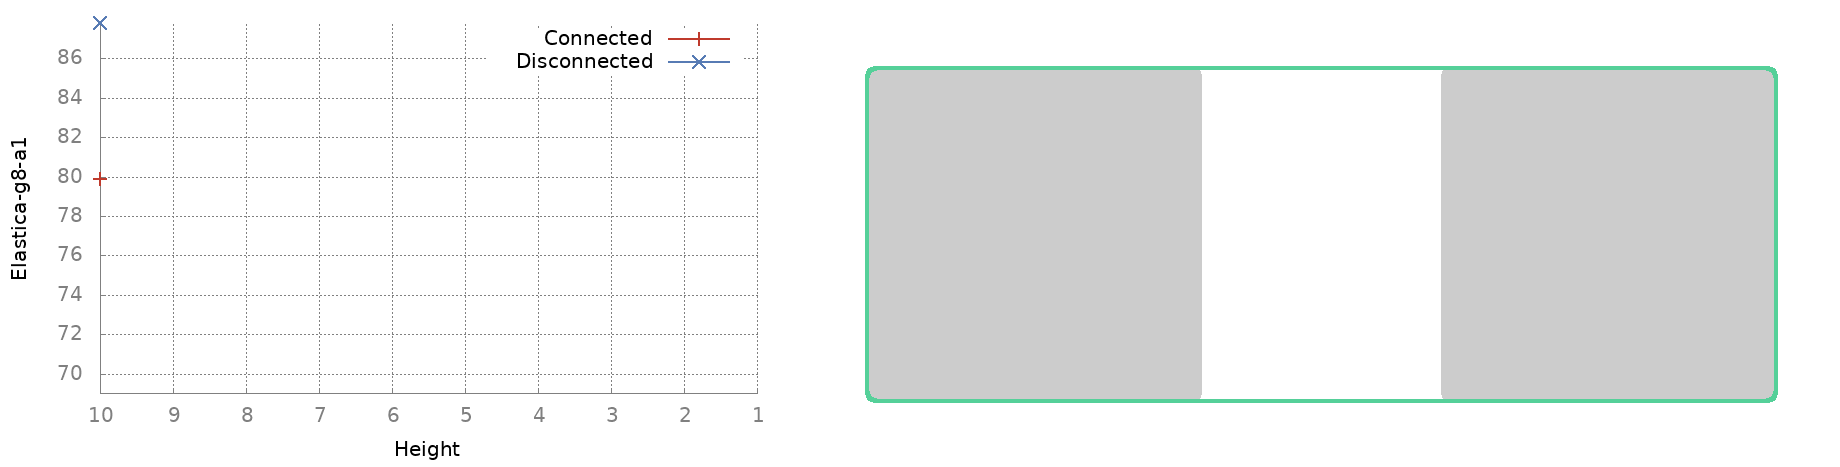
\includegraphics[scale=0.22]{figures/motivation/completion/elastica-g8a1-0.png}
}
\only<2>{
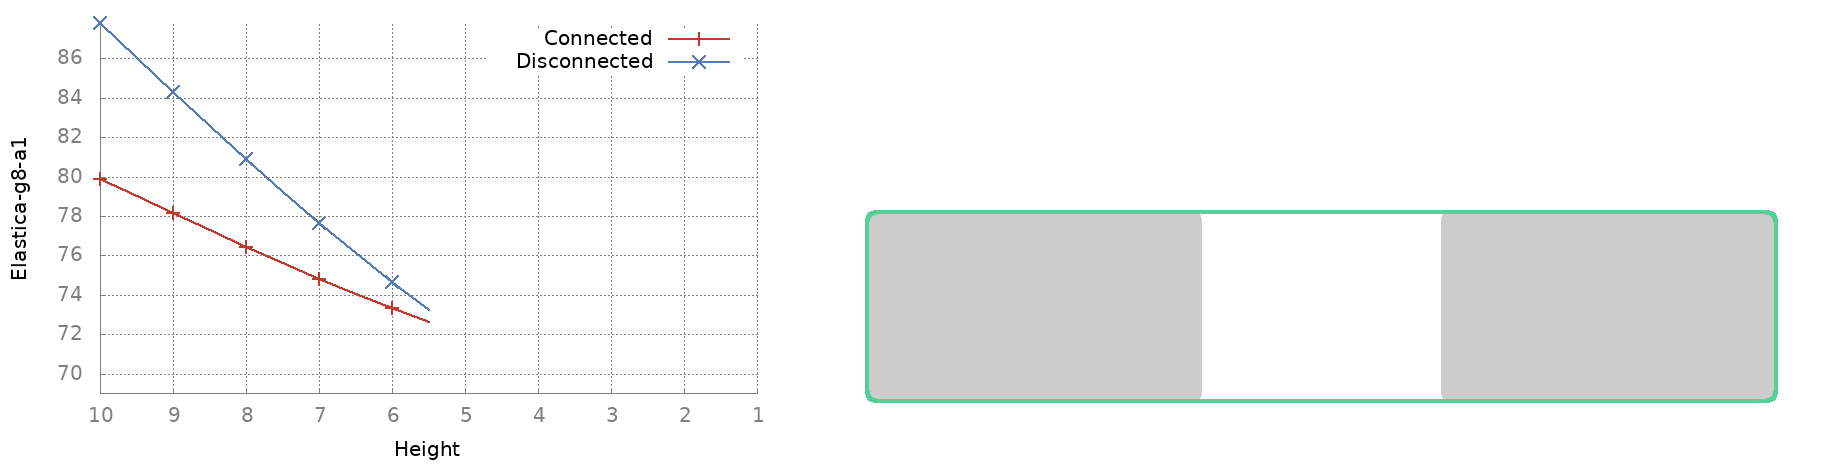
\includegraphics[scale=0.22]{figures/motivation/completion/elastica-g8a1-1.png}
}
\only<3>{
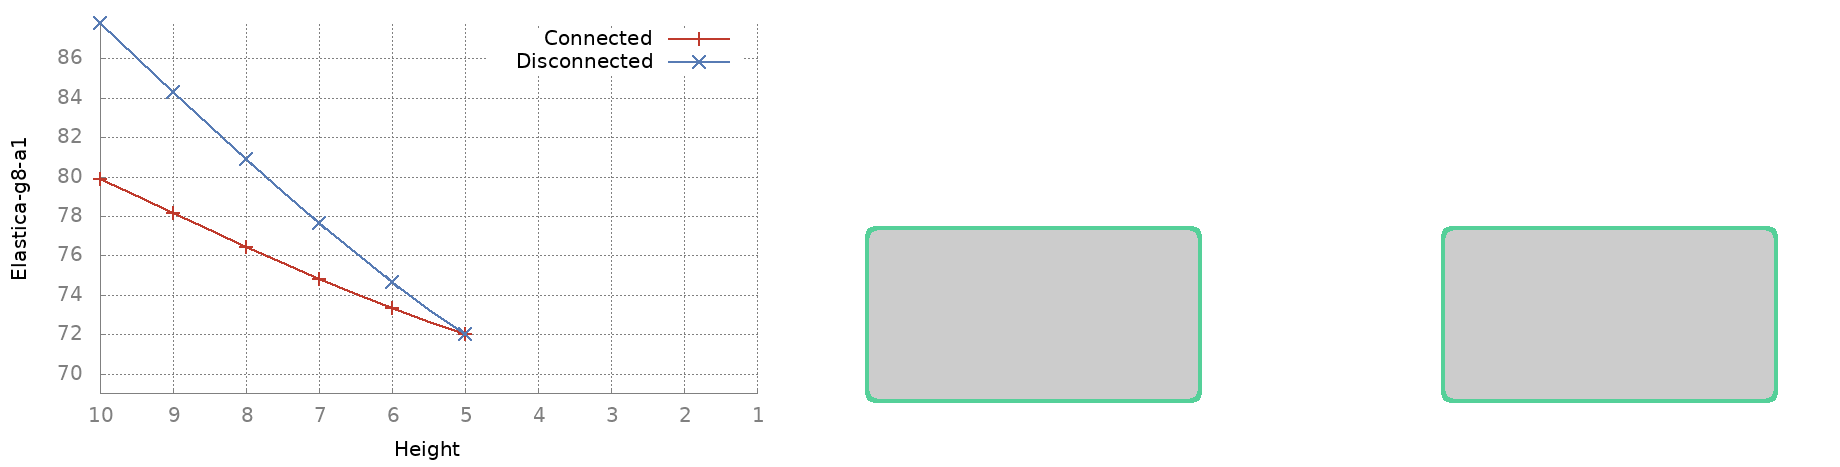
\includegraphics[scale=0.22]{figures/motivation/completion/elastica-g8a1-2.png}
}
\only<4>{
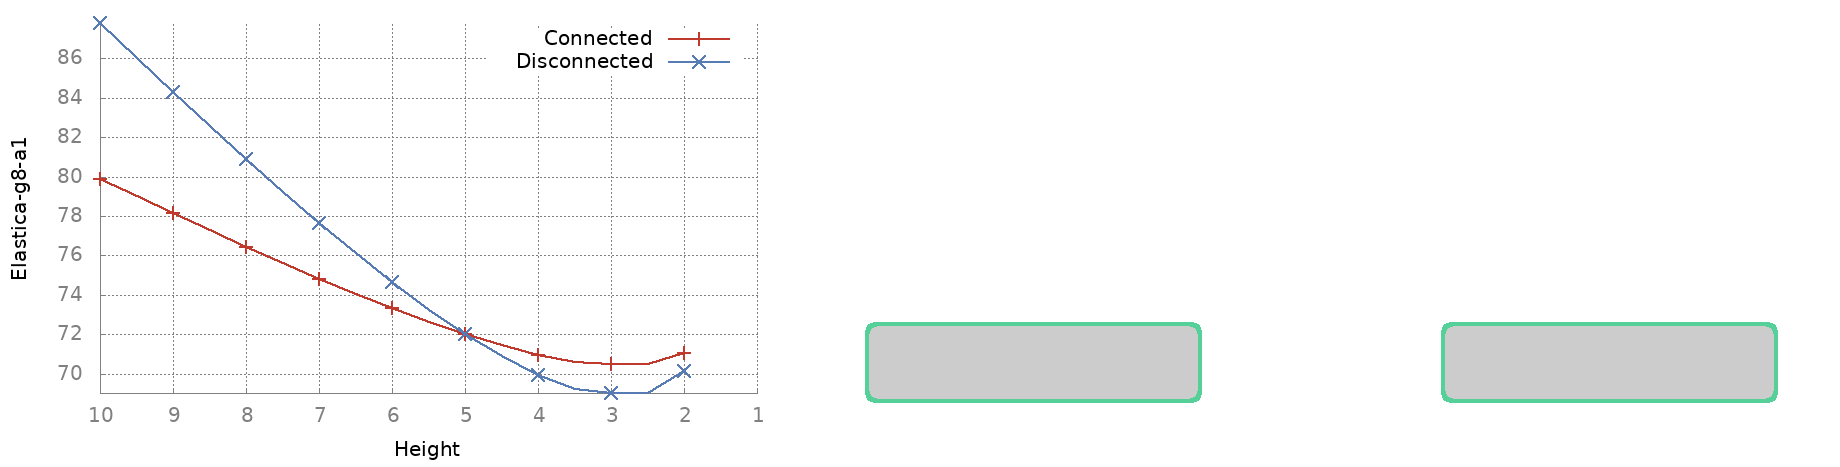
\includegraphics[scale=0.22]{figures/motivation/completion/elastica-g8a1-3.png}
}
\only<5->{
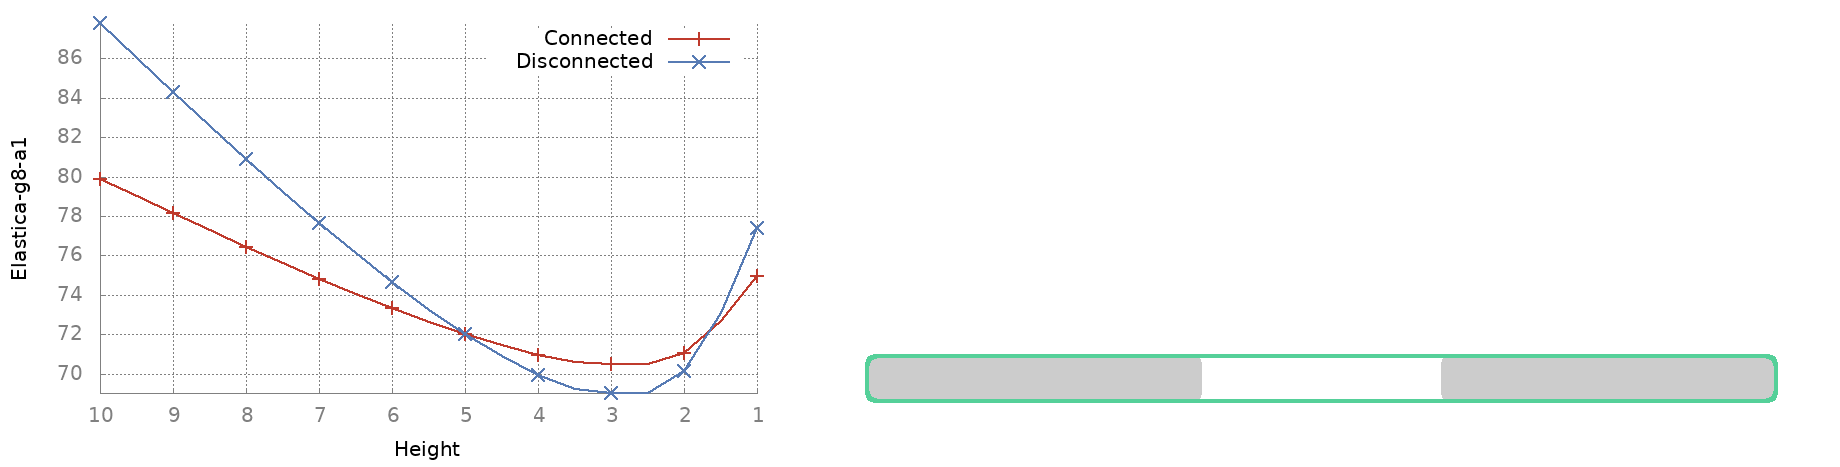
\includegraphics[scale=0.22]{figures/motivation/completion/elastica-g8a1-4.png}
}
\end{minipage}
\begin{minipage}[t][0.5\textheight][t]{\textwidth}
\only<6->{
\center
$\min_{ \Omega \in \{\Omega_{c}, \Omega_{d} \} } \frac{1}{2}\int_{\partial \Omega}{ds} + \int_{\partial \Omega}{ \kappa ^2ds}.$}
\only<6>{
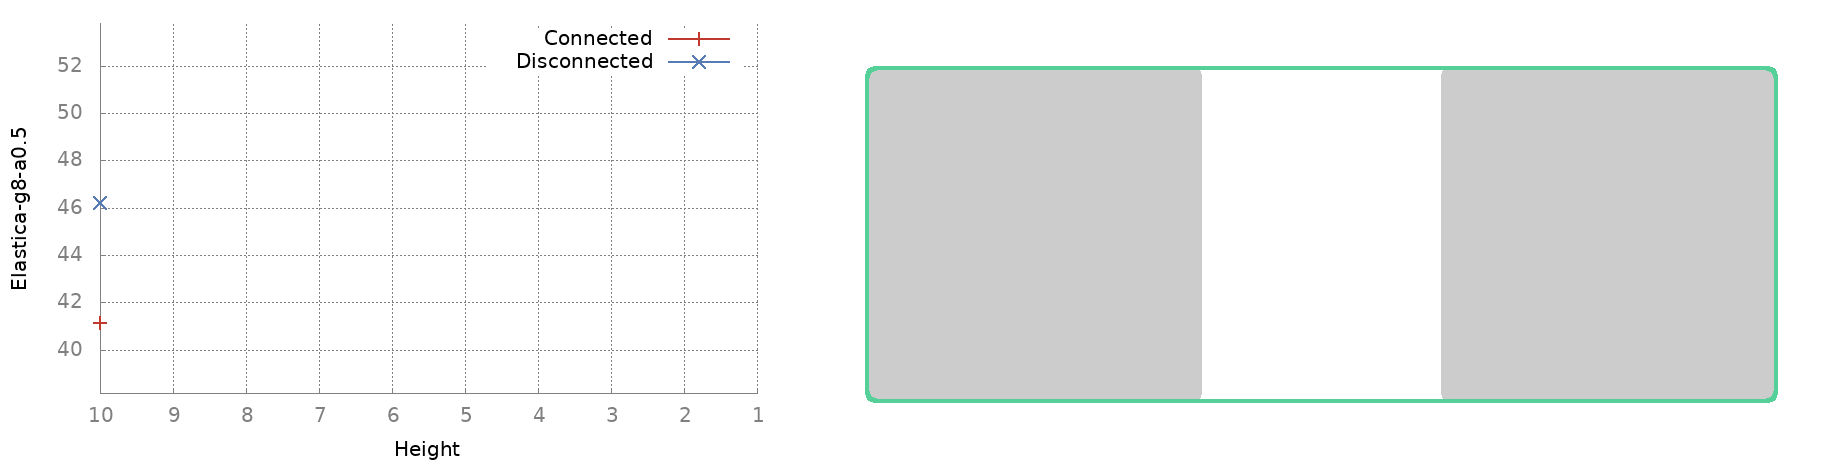
\includegraphics[scale=0.22]{figures/motivation/completion/elastica-g8a05-0.png}
}
\only<7>{
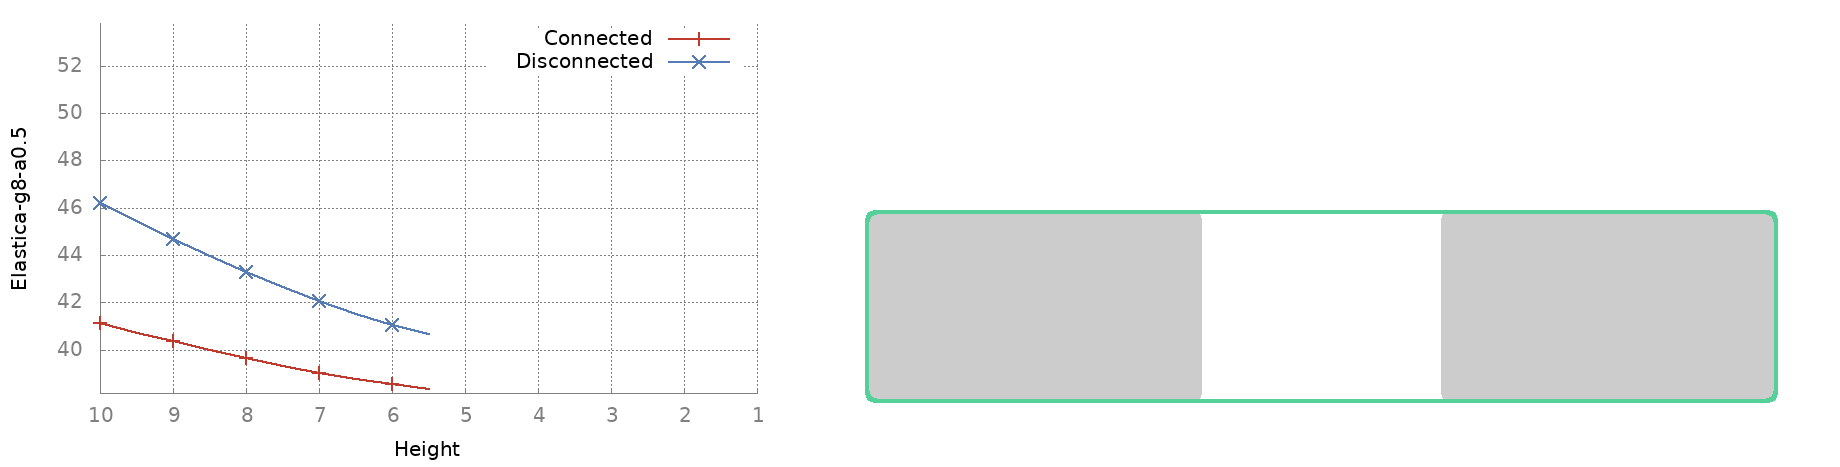
\includegraphics[scale=0.22]{figures/motivation/completion/elastica-g8a05-1.png}
}
\only<8>{
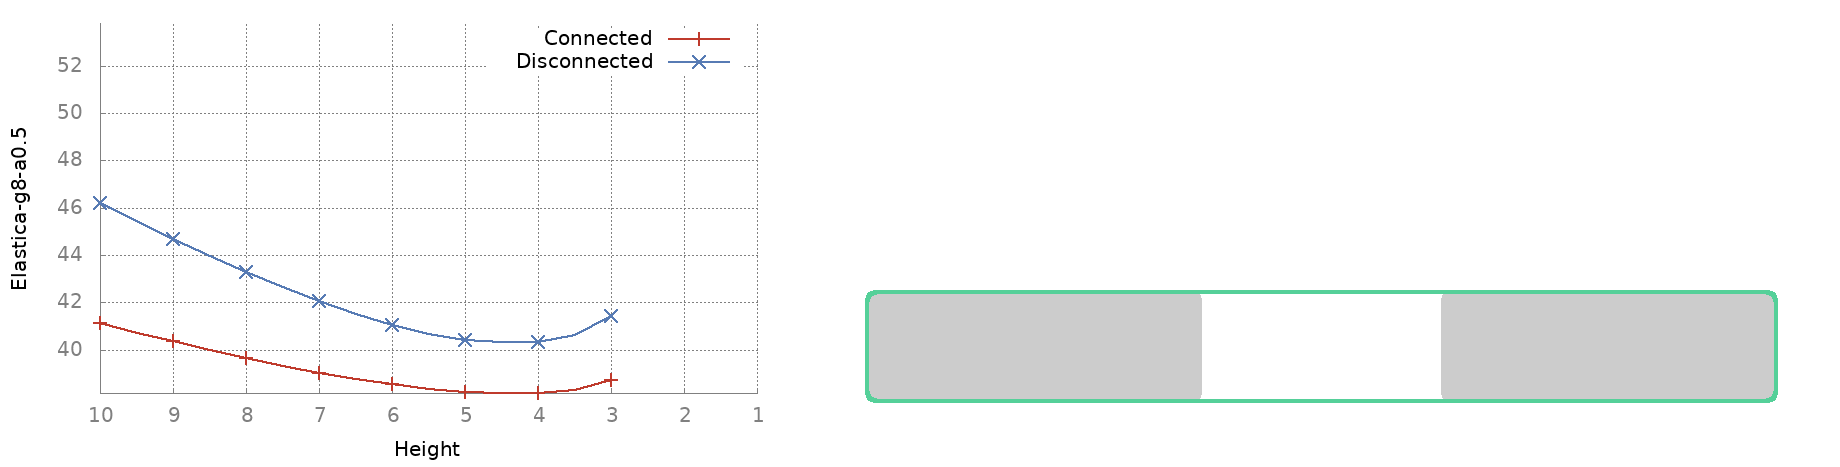
\includegraphics[scale=0.22]{figures/motivation/completion/elastica-g8a05-2.png}
}
\only<9>{
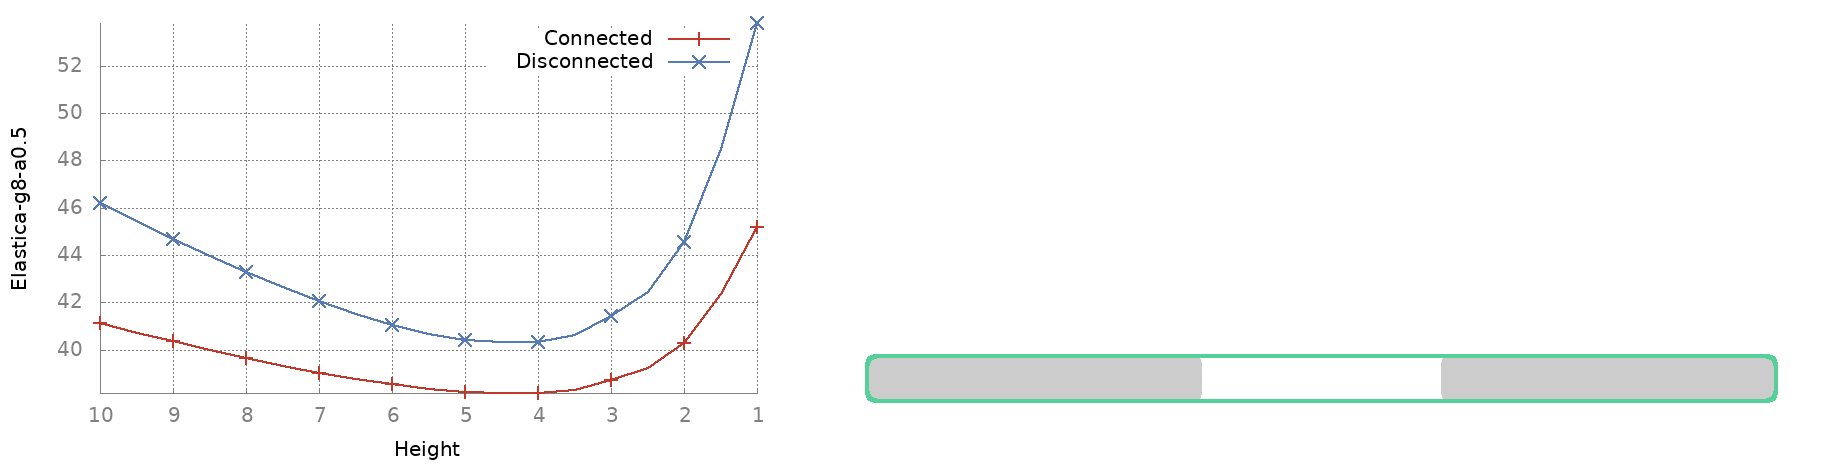
\includegraphics[scale=0.22]{figures/motivation/completion/elastica-g8a05-3.png}
}
\end{minipage}
\end{frame}

\begin{frame}
{Motivation}
{State-of-art}

\textbf{Continuous world}: Define the energy over the whole domain and minimize the elastica with respect the level-curves.
%
\begin{align*}
\int_{\Omega}{ \left(\alpha + \beta \nabla \cdot \left(\frac{\nabla f_{\vec{I}}}{\norm{\nabla f_{\vec{I}} }}\right) ^2 \right)\norm{\nabla f_{\vec{I}} }d\Omega}.
\end{align*}
%
\pause
\begin{itemize}
\item{Numerical instability: Fourth-order Euler-Lagrange equation.}
\item{Subject to bad local minimum.}
\end{itemize}
%
\pause
\vspace{1em}
\textbf{Discrete world}:

\begin{itemize}
\item{T-junctions matching: Fast algorithm, but limited to absolute value of curvature (polygonal solutions) and inpainting application.}\pause
\item{Linear programming formulation: global optimization, but hours of execution using small (thus unprecise) neighborhood.}\pause
\item{Triple cliques: global optimization, non-submodular energy. Limited precision.}
\end{itemize}
\end{frame}

\begin{frame}
{Motivation}
{Digital set peculiarities}

\textbf{Exact sampling x digitization}

\begin{minipage}{0.3\textwidth}
\center
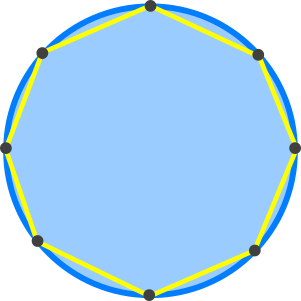
\includegraphics[scale=0.45]{figures/motivation/exact-sampling/sampling-0.png}
\end{minipage}
\begin{minipage}{0.3\textwidth}
\center
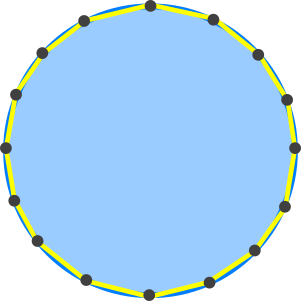
\includegraphics[scale=0.45]{figures/motivation/exact-sampling/sampling-1.png}
\end{minipage}
\begin{minipage}{0.3\textwidth}
\center
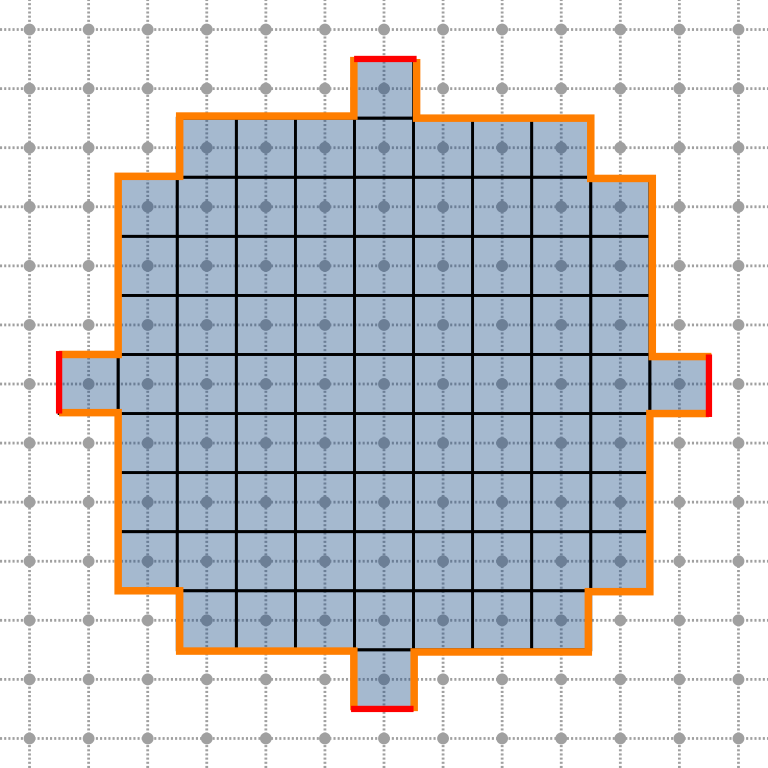
\includegraphics[scale=0.22]{figures/motivation/exact-sampling/digital-ball-perimeter.png}
\end{minipage}
\vspace{1em}
%
\pause
%
\textbf{Digitization ambiguity}
\begin{center}
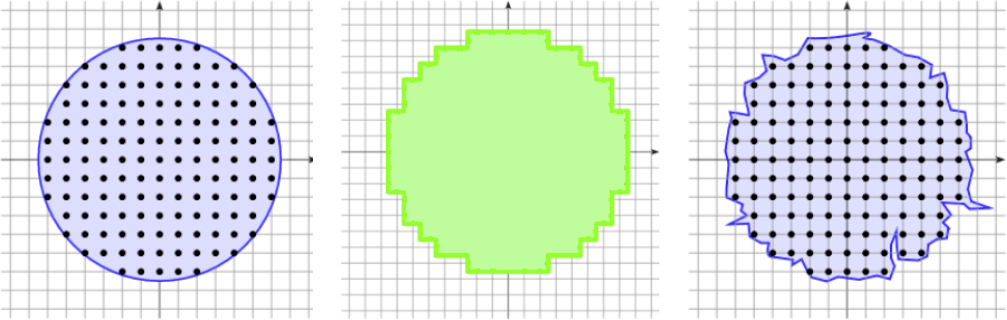
\includegraphics[scale=1]{figures/motivation/exact-sampling/ambiguity.png}
\end{center}
\end{frame}

\begin{frame}
{Motivation}
{Multigrid convergent estimators}

\begin{definition}[Multigrid convergence]
	Let $\mathcal{X}$ be a family of shapes in $\mathbb{R}^n$ and $u$ a geometric quantity that is defined for every shape $X \in \mathcal{X}$. Further, let $D_h(X)$ denote the digitization of $X$ with grid step $h$.%
%
\vspace{1em}	
%	
	 The estimator $\hat{u}$ is multigrid convergent for $\mathcal{X}$ if and only if, for any $X \in \mathcal{X}$ there exists $h_X > 0$ such that for every $0< h < h_X$
	
	\begin{align*}
		| \hat{u}(D_h(X)) - u(X) | \leq \tau(h), \quad \text{with } \lim_{h\rightarrow 0}{\tau(h)} = 0
	\end{align*}	
\end{definition}
%
\pause
%
Multigrid convergent estimator of area
\begin{align*}
	\widehat{Area(X)} = h^2|D_h(X)|
\end{align*}
%
\end{frame}

\begin{frame}
	{Motivation}	
	{Multigrid convergent estimators}
	
	Examples of multigrid convergent estimators of perimeter (for piecewise $3$-smooth convex shapes).
%
	\vspace{2em}	
%
	\begin{itemize}
		\onslide<1->{\item{Minimum Length Polygon (MLP)
			\item[]{ \small \citet*{sloboda98mlp}}}}
		\onslide<3->{\item{$\lambda$-Maximal Segment Tangent ($\lambda$-MST) 
			\item[]{\small \citet*{lachaud07tangent}}}}
	\end{itemize}
	
	\onslide<2>{
	\begin{figure}
	\begin{tikzpicture}[overlay, remember picture] 
	\node at (current page.center) 
	    [
	    anchor=center,
	    xshift=0mm,
	    yshift=0mm
	    ] 
	{
	
	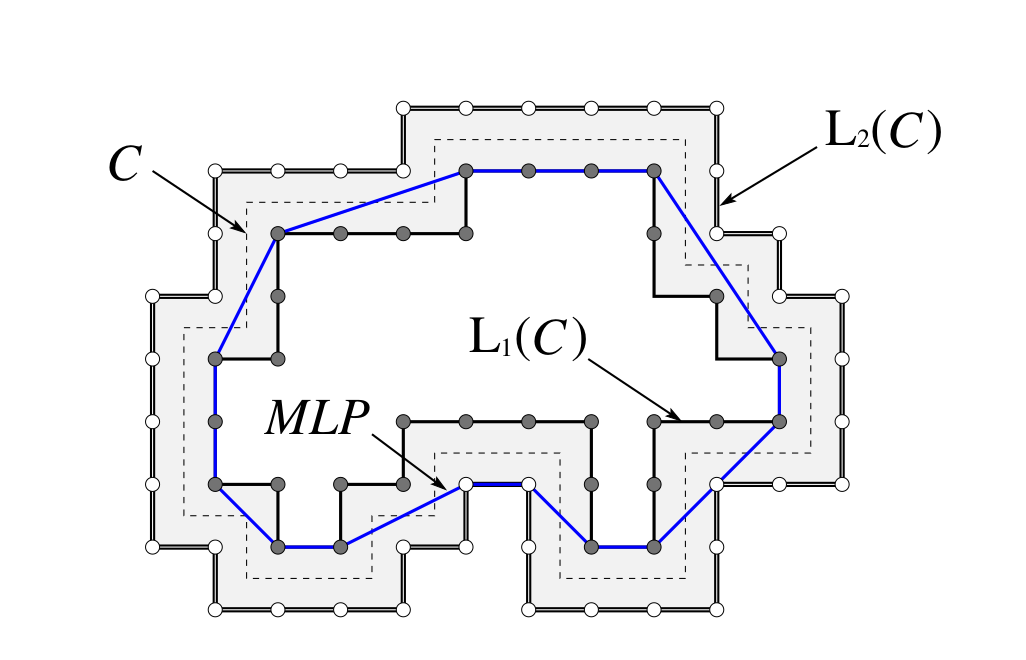
\includegraphics[scale=1.0]{figures/motivation/digital-geometric-estimators/mlp.png}
		
	};
	\end{tikzpicture}	
	\end{figure}	
	}
	
	\onslide<4>{
	\begin{figure}
	\begin{tikzpicture}[overlay, remember picture] 
	\node at (current page.center) 
	    [
	    anchor=center,
	    xshift=0mm,
	    yshift=0mm
	    ] 
	{
	
	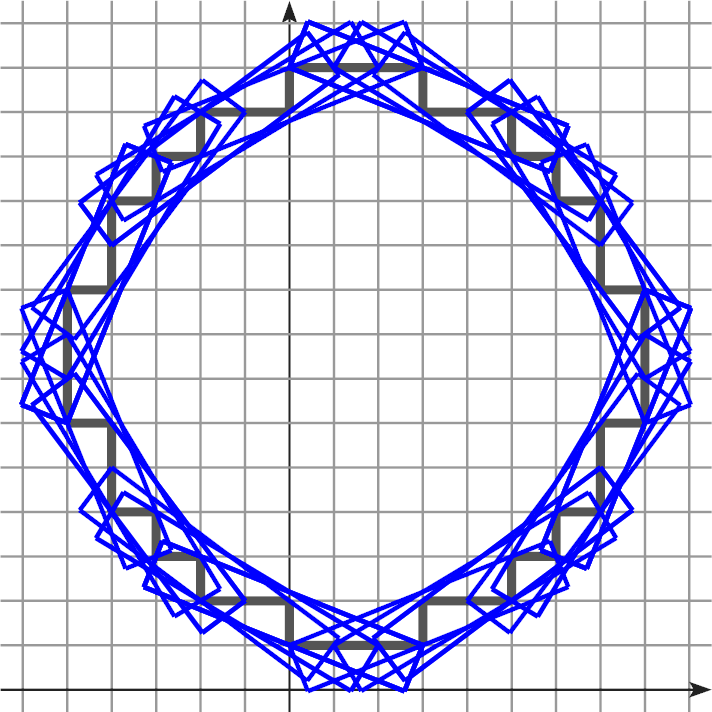
\includegraphics[scale=1.0]{figures/motivation/digital-geometric-estimators/tangential-cover.png}
		
	};
	\end{tikzpicture}	
	\end{figure}	
	}	
	
	
\end{frame}

\begin{frame}
	{Motivation}	
	{Digital geometric estimator}
	
	Examples of multigrid convergent estimators of curvature:
	\begin{itemize}
		\onslide<1->{\item{$\lambda$-Maximal Digital Circular Arcs ($\lambda$-MDCA)
		\item[]{\small \citet*{roussillon11mdca}}
		\item[]{\small \citet*{schindele17}}}
		\begin{itemize}
			\item{Proved multigrid convergent for convex shapes with continuous curvature.}
		\end{itemize}				
		
		}
		\onslide<3->{\vspace{2em}
		\item{Integral Invariant (II)}
		\item[]{\small \citet*{coeurjolly13integral}}
		\begin{itemize}
			\item{Proved multigrid convergent for $C^2$ convex shapes with bounded curvature.}
		\end{itemize}				
		}
	\end{itemize}	
	
	\onslide<2>{
	\begin{figure}
	\begin{tikzpicture}[overlay, remember picture] 
	\node at (current page.center) 
	    [
	    anchor=center,
	    xshift=0mm,
	    yshift=0mm
	    ] 
	{
	
	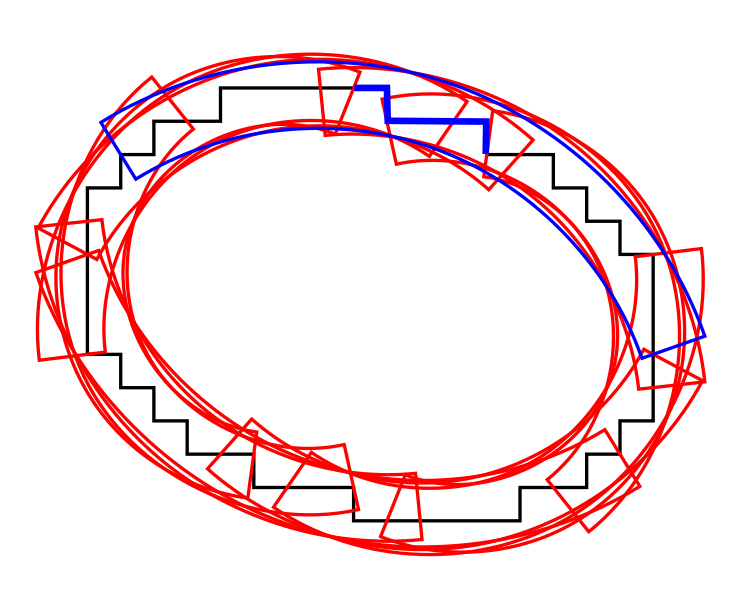
\includegraphics[scale=1.0]{figures/motivation/digital-geometric-estimators/mdca.png}
		
	};
	\end{tikzpicture}	
	\end{figure}	
	}		
	
	\onslide<4>{
	\begin{figure}
	\begin{tikzpicture}[overlay, remember picture] 
	\node at (current page.center) 
	    [
	    anchor=center,
	    xshift=0mm,
	    yshift=0mm
	    ] 
	{
	
	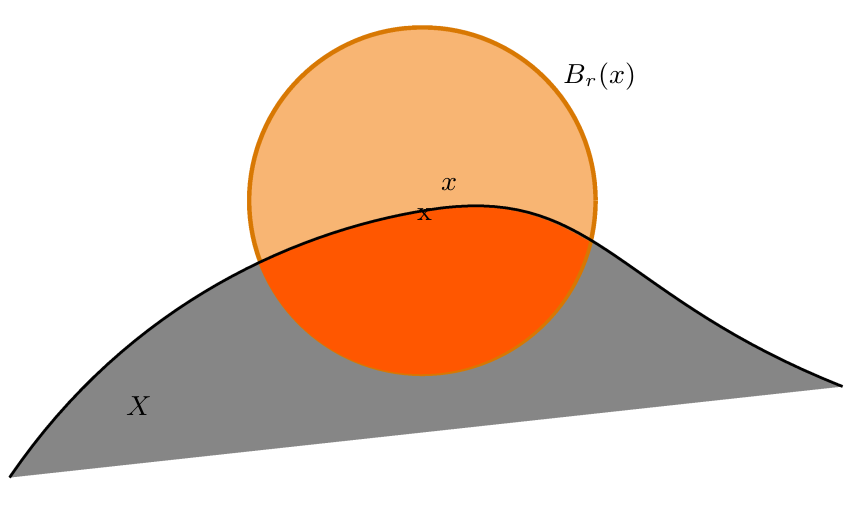
\includegraphics[scale=1.0]{figures/motivation/digital-geometric-estimators/ii.png}
		
	};
	\end{tikzpicture}	
	\end{figure}	
	}	
	
	\onslide<4>{
	\begin{align*}
		\hat{\kappa}(p) = \frac{3}{r^3}\left( \frac{\pi r^2}{2} - | B_r(p) \cap X | \right )
	\end{align*}}	
	
	
\end{frame}

\begin{frame}
{Motivation}
{Goals}

\begin{itemize}
\item{Can we define an elastica-based model for image analysis using multigrid convergent estimators? \only<4>{\color{green}Yes!}} \pause
\item{Can we recover the completion property of elastica? \only<4>{\color{green}Yes!}} \pause
\item{Can we escape bad local minima? \only<4>{\color{green}Yes!}}
\end{itemize}

\end{frame}